% electrostatica-002.tex
%
% Copyright (C) 2019-2025 José A. Navarro Ramón <janr.devel@gmail.com>
% .............................................................................
% OBSERVACIÓN: Se puede dar formato al búffer en AUCTeX con: M-x L-buff RET
% .............................................................................

\documentclass[a4paper,10pt]{article}

\usepackage{../edclasica-res.pkg}
\usepackage{../edclasica-res.defs}

% *****************************************************************************
% ******* DEFINICIONES DE ESTE EJERCICIO **************************************
% *****************************************************************************
% Bloques de ejercicios
\renewcommand*{\mainsubject}{Electrostática}
\renewcommand*{\parte}{EJERCICIOS DE ELECTRODINÁMICA CLÁSICA}
\renewcommand*{\tipoBloque}{Problema}
\renewcommand*{\bloque}{2}
\renewcommand*{\hoja}{1}
\renewcommand*{\ejBloque}{2}
% Fuente: examen
%\renewcommand*{\ejExamen}{1}
\renewcommand*{\fuente}{Introduction to Electrodynamics - Griffiths - 4th Ed.
  Exercise 2.2. Page 61.}

\def\rcurs{{\mbox{$\resizebox{.09in}{.08in}
      {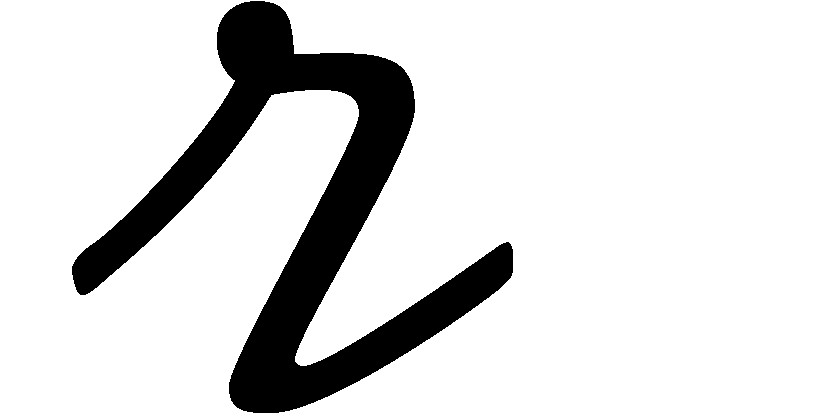
\includegraphics[trim= 1em 0 14em 0,clip]{ScriptR}}$}}}
\def\brcurs{{\mbox{$\resizebox{.09in}{.08in}
      {
\includegraphics[trim= 1em 0 14em 0,clip]{BoldR}}$}}}
\def\hrcurs{{\mbox{$\hat \brcurs$}}}

% $\brcurs$ --> Vector separación.
% $\rcurs$ --> Módulo del vector separación.
% $\hrcurs$ --> Vector unitario separación.
%  $\hrcurs_{1}/\rcurs_{1}^{2}$

% *****************************************************************************

\begin{document}

% ############################ ENUNCIADO ######################################
% Entrada en el índice del fichero 'pdf' 'enunciado.0'
\pdfbookmark[0]{Enunciado}{enunciado}

% -----------------------------------------------------------------------------
% 
% -----------------------------------------------------------------------------
%\item[\ejBloque.-]~\\[-3.0em]
\begin{qboxshort}
    Calcule el campo eléctrico (módulo, dirección y sentido) a una distancia
    $z$ sobre el punto medio que hay entre dos cargas iguales y opuestas
    ($\pm q$) a una distancia $d$ entre ellas. La carga en la posición
    $x= +d/2$ es $-q$.
\end{qboxshort}

% ######################### RESOLUCIÓN ########################################

% Entrada en el índice del fichero 'pdf'
\pdfbookmark[0]{Solución}{sol}

\begin{soluc}
\item En las figuras~\ref{fig:vectores1} y \ref{fig:vectores2} se
  representan dos cargas iguales y opuestas sobre el eje $x$. Nos
  proponemos calcular el campo eléctrico en un punto $P$ situado a una
  distancia $z$ por encima del punto medio entre las cargas.

  El campo eléctrico creado por una carga puntual en un punto con vector
  de posición $\vvv{r}$ es
  \[
    \vvv{E}(\vvv{r})
    = \dfrac{1}{4\pi\epsilon_{0}}\,
    \dfrac{q}{\rcurs^{2}}\,\hrcurs
  \]
  donde $\brcurs = \vvv{r} - \vvv{r}'$, siendo $\vvv{r}$ el vector posición
del punto donde se calcula el campo y $\vvv{r}'$ el vector posición de la
carga, como se puede apreciar en las figuras.

  \begin{figure}[ht]
    \def\scl{1}
    \def\equis{1.5}
    \def\xeje{3.0}
    \def\zeje{4.0}
    \def\angref{60}
    \def\vectlen{1.8}
    \centering
    \begin{minipage}{0.37\linewidth}
    \begin{tikzpicture}[scale=\scl]
      % Coordenadas
      \coordinate (O) at (0,0);
      \coordinate (xm) at (-\equis,0);
      \coordinate (xp) at (\equis,0);
      \path[name path=linea a] (xp) -- +(180-\angref:6);
      % Ejes
      \draw[-{Latex}] (-\xeje,0) -- (\xeje,0)
      node[anchor=north west] {$x$};
      \draw[-{Latex},name path=linea z]
      (O) -- (0,\zeje) node[anchor=south east] {$z$};
      % Cargas
      \filldraw[fill=red,draw=black] (xp) circle [radius=2pt];
      \filldraw[fill=red,draw=black] (xm) circle [radius=2pt];
      
      \node[below right=2pt and 0pt] at (xp) {$q_{1}$};
      \node[below left=2pt and 0pt] at (xm) {$q_{2}$};
      %\path[anchor=north] (O) -- node {$+\frac{d}{2}$} (xp);
      %\path[anchor=north] (O) -- node {$-\frac{d}{2}$} (xm);
      % Punto z
      \path [name intersections={of=linea a and linea z, by=z}];
      %\path[anchor=east] (O) -- node {$z$} (z);
      % Vectores de posición
      \draw[-{Latex[round]},ultra thick,shorten >=3pt]
      (O) -- node[left] {$\vvv{r}$} (z);
      \draw[-{Latex[round]},ultra thick,shorten >=3pt]
      (O) --node[below] {$\vvv{r}'_{1}$}(xp);
      \draw[-{Latex},ultra thick,shorten >=2pt] (xp) --
      node[anchor=south west] {$\brcurs_{1} = \vvv{r}-\vvv{r}_{1}'$}(z);

      % Punto z y Origen y Cargas
      \filldraw[fill=black,draw=black] (z) circle [radius=2pt];
      \node[black,anchor=south east] at (z) {$P$};
      \filldraw[fill=black,draw=black] (O) circle [radius=2pt];
      \node[black,below=1pt] at (O) {$O$};
      \filldraw[fill=red,draw=black] (xp) circle [radius=2pt];
      %\node[black] at (xp) {\textbf{$-$}};
      \filldraw[fill=green,draw=black] (xm) circle [radius=2pt];
      %\node[black] at (xm) {\textbf{$+$}};
    \end{tikzpicture}%
    \caption{Vectores que intervienen en el cálculo del campo electrico
    creado por la carga $q_{1}$.}
    \label{fig:vectores1}
\end{minipage}%
%
\hskip 5em%
%
\begin{minipage}{0.37\linewidth}
    \begin{tikzpicture}[scale=\scl]
      % Coordenadas
      \coordinate (O) at (0,0);
      \coordinate (xm) at (-\equis,0);
      \coordinate (xp) at (\equis,0);
      \path[name path=linea a] (xp) -- +(180-\angref:6);
      % Ejes
      \draw[-{Latex}] (-\xeje,0) -- (\xeje,0)
      node[anchor=north west] {$x$};
      \draw[-{Latex},name path=linea z]
      (O) -- (0,\zeje) node[anchor=south east] {$z$};
      % Cargas
      \filldraw[fill=red,draw=black] (xp) circle [radius=2pt];
      \filldraw[fill=red,draw=black] (xm) circle [radius=2pt];
      
      \node[below right=2pt and 0pt] at (xp) {$q_{1}$};
      \node[below left=2pt and 0pt] at (xm) {$q_{2}$};

      % Punto z
      \path [name intersections={of=linea a and linea z, by=z}];
      
      % Vectores de posición
      \draw[-{Latex[round]},ultra thick,shorten >=3pt]
      (O) -- node[right] {$\vvv{r}$} (z);
      \draw[-{Latex[round]},ultra thick,shorten >=3pt]
      (O) --node[below] {$\vvv{r}'_{2}$}(xm);
      \draw[-{Latex},ultra thick,shorten >=2pt] (xm) --
      node[anchor=south east] {$\brcurs_{2} = \vvv{r}-\vvv{r}_{2}'$}(z);

      % Punto z y Origen y Cargas
      \filldraw[fill=black,draw=black] (z) circle [radius=2pt];
      \node[black,anchor=south east] at (z) {$P$};
      \filldraw[fill=black,draw=black] (O) circle [radius=2pt];
      \node[black,below=1pt] at (O) {$O$};
      \filldraw[fill=red,draw=black] (xp) circle [radius=2pt];
      %\node[black] at (xp) {\textbf{$-$}};
      \filldraw[fill=green,draw=black] (xm) circle [radius=2pt];
      %\node[black] at (xm) {\textbf{$+$}};
    \end{tikzpicture}%
    \caption{Vectores que intervienen en el cálculo del campo electrico
    creado por la carga $q_{s}$.}
    \label{fig:vectores2}
\end{minipage}
\end{figure}

El campo eléctrico total en $P$, con vector posición $\vvv{r}$, es la
resultante de los campos eléctricos creados por las dos cargas
$q_{1}=-q$ y $q_{2}=+q$. 

\begin{itemize}
\item Campo eléctrico $\vvv{E}_{1}$ en $P$ creado por la carga $q_{1}=-q$.
  Los vectores relevantes para el cálculo se representan en la
  figura~\ref{fig:vectores1}. Utilizamos la misma para calcular
  los vectores $\brcurs_{1}$, $\rcurs_{1}$, $\hrcurs_{1}$ y
  $\hrcurs_{1}/\rcurs_{1}^{2}$
\begin{align*}
  \brcurs_{1}
  &=
    \vvv{r} - \vvv{r}'_{1}
    =
    z\,\xhat{u}_{z} - \frac{d}{2}\,\xhat{u}_{x}\\
  \hrcurs_{1}
  &=
    \frac{\brcurs_{1}}{\rcurs_{1}}
    =
    \frac{z\,\xhat{u}_{z} - \frac{d}{2}\,\xhat{u}_{x}}
    {\sqrt{z^{2}+\left(-\frac{d}{2}\right)^{2}}}
    =
    \frac{z\,\xhat{u}_{z} - \frac{d}{2}\,\xhat{u}_{x}}
    {\left(z^{2}+\frac{d^{2}}{4}\right)^{1/2}}
    =
    \frac{z}{\left(z^{2}+\frac{d^{2}}{4}\right)^{1/2}}\,\xhat{u}_{z}
    -
    \frac{d/2}{\left(z^{2}+\frac{d^{2}}{4}\right)^{1/2}}\,\xhat{u}_{x}\\
    \frac{\hrcurs_{1}}{\rcurs_{1}^ {2}}
  &=
    \frac{\brcurs_{1}/\rcurs_{1}}{\rcurs_{1}^{2}}
    =
    \frac{\brcurs_{1}}{\rcurs_{1}^{3}}
    =
    \frac{z\,\xhat{u}_{z} - \frac{d}{2}\,\xhat{u}_{x}}
    {\left(\sqrt{z^{2}+\left(-\dfrac{d}{2}\right)^{2}}\right)^{3}}
    =
    \frac{z\,\xhat{u}_{z} - \frac{d}{2}\,\xhat{u}_{x}}
    {\left(z^{2}+\dfrac{d^{2}}{4}\right)^{3/2}}
\end{align*}
donde $\xhat{u}_{x}$ y $\xhat{u}_{z}$ son los vectores unitarios en
los ejes $x$ y $z$, respectivamente.

Entonces $\vvv{E}_{1}$ queda
\begin{equation}\label{eq:E1}
  \vvv{E}_{1}
  =
  \frac{q_{1}}{4\pi\epsilon_{0}}\,\frac{\hrcurs_{1}}{\rcurs_{1}^{2}}
  =
  \frac{-q}{4\pi\epsilon_{0}}\,
  \frac{z\,\xhat{u}_{z} - \frac{d}{2}\,\xhat{u}_{x}}
  {\left(z^{2}+\dfrac{d^{2}}{4}\right)^{3/2}}
  =
  \frac{q}{4\pi\epsilon_{0}}\,
  \frac{-z\,\xhat{u}_{z} + \frac{d}{2}\,\xhat{u}_{x}}
  {\left(z^{2}+\dfrac{d^{2}}{4}\right)^{3/2}}  
\end{equation}

\item Campo eléctrico $\vvv{E}_{2}$ en $P$ creado por la carga $q_{2}=+q$.
  Los vectores relevantes para el cálculo se representan en la
  figura~\ref{fig:vectores2}. Utilizamos la misma para calcular los
  vectores $\brcurs_{2}$, $\rcurs_{2}$, $\hrcurs_{2}$ y
  $\hrcurs_{2}/\rcurs_{2}^{2}$
\begin{align*}
  \brcurs_{2}
  &=
    \vvv{r} - \vvv{r}'_{2}
    =
    z\,\xhat{u}_{z} - \left(-\frac{d}{2}\,\xhat{u}_{x}\right)
    =
    z\,\xhat{u}_{z} + \frac{d}{2}\,\xhat{u}_{x}\\
  \hrcurs_{2}
  &=
    \frac{\brcurs_{2}}{\rcurs_{2}}
    =
    \frac{z\,\xhat{u}_{z} + \frac{d}{2}\,\xhat{u}_{x}}
    {\sqrt{z^{2}+\left(\frac{d}{2}\right)^{2}}}
    =
    \frac{z\,\xhat{u}_{z} + \frac{d}{2}\,\xhat{u}_{x}}
    {\left(z^{2}+\frac{d^{2}}{4}\right)^{1/2}}
    =
    \frac{z}{\left(z^{2}+\frac{d^{2}}{4}\right)^{1/2}}\,\xhat{u}_{z}
    +
    \frac{d/2}{\left(z^{2}+\frac{d^{2}}{4}\right)^{1/2}}\,\xhat{u}_{x}\\
    \frac{\hrcurs_{2}}{\rcurs_{2}^ {2}}
  &=
    \frac{\brcurs_{2}/\rcurs_{2}}{\rcurs_{2}^{2}}
    =
    \frac{\brcurs_{2}}{\rcurs_{2}^{3}}
    =
    \frac{z\,\xhat{u}_{z} - \frac{d}{2}\,\xhat{u}_{x}}
    {\left(\sqrt{z^{2}+\left(-\dfrac{d}{2}\right)^{2}}\right)^{3}}
    =
    \frac{z\,\xhat{u}_{z} - \frac{d}{2}\,\xhat{u}_{x}}
    {\left(z^{2}+\dfrac{d^{2}}{4}\right)^{3/2}}
\end{align*}
donde $\xhat{u}_{x}$ y $\xhat{u}_{z}$ son los vectores unitarios en
los ejes $x$ y $z$, respectivamente.

Entonces $\vvv{E}_{2}$ queda
\begin{equation}\label{eq:E2}
  \vvv{E}_{2}
  =
  \frac{q_{2}}{4\pi\epsilon_{0}}\,\frac{\hrcurs_{2}}{\rcurs_{2}^{2}}
  =
  \frac{q}{4\pi\epsilon_{0}}\,
  \frac{z\,\xhat{u}_{z} + \frac{d}{2}\,\xhat{u}_{x}}
  {\left(z^{2}+\dfrac{d^{2}}{4}\right)^{3/2}}
  =
  \frac{q}{4\pi\epsilon_{0}}\,
  \frac{z\,\xhat{u}_{z} + \frac{d}{2}\,\xhat{u}_{x}}
  {\left(z^{2}+\dfrac{d^{2}}{4}\right)^{3/2}}  
\end{equation}

\end{itemize}


\begin{figure}[ht]
    \def\scl{1}
    \def\equis{1.5}
    \def\xeje{3.0}
    \def\zeje{4.0}
    \def\angref{60}
    \def\vectlen{1.8}
\begin{minipage}{.38\linewidth}
   \begin{tikzpicture}[scale=\scl, baseline]
      % Coordenadas
      \coordinate (O) at (0,0);
      \coordinate (xm) at (-\equis,0);
      \coordinate (xp) at (\equis,0);
      \path[name path=linea a] (xp) -- +(180-\angref:6);
      % Ejes
      \draw[-{Latex}] (-\xeje,0) -- (\xeje,0) node[anchor=north west] {$x$};
      \draw[-{Latex},name path=linea z]
      (O) -- (0,\zeje) node[anchor=south east] {$z$};
      % Cargas
      \filldraw[fill=red,draw=black] (xp) circle [radius=2pt];
      \filldraw[fill=red,draw=black] (xm) circle [radius=2pt];
      
      \node[below right=2pt and 0pt] at (xp) {$q_{1}$};
      \node[below left=2pt and 0pt] at (xm) {$q_{2}$};
      \path[anchor=north] (O) -- node {$+\frac{d}{2}$} (xp);
      \path[anchor=north] (O) -- node {$-\frac{d}{2}$} (xm);
      % Punto z
      \path [name intersections={of=linea a and linea z, by=z}];
      \path[anchor=east] (O) -- node {$z$} (z);
      % Vectores
      \draw[-{Latex},red!50!black,ultra thick] (z) --
      ++(-\angref:\vectlen)
      coordinate (E1);
      \node[anchor=north east,black] at (E1) {$\vvv{E}_{1}$};
      \draw[-{Latex},green!40!black,ultra thick] (z) --
      ++(\angref:\vectlen)
      coordinate (E2);
      \node[anchor=south east,black] at (E2) {$\vvv{E}_{2}$};
      % Líneas auxiliares de vectores
      \draw[ultra thin,black!50] (E1) -- ++(\angref:\vectlen)
      coordinate (E);
      \draw[ultra thin,black!50] (E2) -- ++(-\angref:\vectlen);
      % Vector resultante
      \draw[-{Latex},black,ultra thick] (z) -- (E);
      \node[anchor=west] at (E) {$\vvv{E}$};

      % Punto z y Cargas
      \filldraw[fill=black,draw=black] (z) circle [radius=2pt];
      \node[black, anchor=south east] at (z) {$P$};
      \filldraw[fill=red!40,draw=black] (xp) circle [radius=5pt];
      \node[black] at (xp) {\raisebox{-5pt}{\textbf{$-$}}};
      \filldraw[fill=green!40,draw=black] (xm) circle [radius=5pt];
      \node[black] at (xm) {\textbf{$+$}};
  \end{tikzpicture}%
  \caption{Dos cargas iguales y opuestas $\pm q$ están situadas sobre el
    eje $x$ a una distancia $d$ entre ellas. El campo eléctrico $\vvv{E}$ a
    una distancia $z$ sobre el punto medio entre las dos cargas es la suma
    de los campos eléctricos creados por cada carga en dicho punto,
    $\vvv{E_{1}}$ y $\vvv{E_{2}}$.}
\label{fig:cargas-iguales-y-opuestas}
\end{minipage}%
%
\hskip 3em%
%
\begin{minipage}{.55\linewidth}
  Aplicamos el \emph{principio de superposición} para calcular el campo
  eléctrico total en $P$, utilizando los valores hallados para $\vvv{E}_{1}$
  y $\vvv{E}_{2}$ en las ecuaciones~(\ref{eq:E1}) y (\ref{eq:E2}),
  respectivamente
  \begin{align*}
    \vvv{E}
    &=
      \vvv{E}_{1} + \vvv{E}_{2}
      =
      \frac{q}{4\pi\epsilon_{0}}\,
      \frac{\cancelout{-z\,\xhat{u}_{z}} + \frac{d}{2}\,\xhat{u}_{x}}
      {\left(z^{2}+\dfrac{d^{2}}{4}\right)^{3/2}}  
      +
      \frac{q}{4\pi\epsilon_{0}}\,
      \frac{\cancelout{z\,\xhat{u}_{z}} + \frac{d}{2}\,\xhat{u}_{x}}
      {\left(z^{2}+\dfrac{d^{2}}{4}\right)^{3/2}}      
  \end{align*}
  El campo eléctrico queda
  \begin{equation}\label{eq:E}
    \vvv{E}
    =
    \frac{1}{4\pi\epsilon_{0}}\,
    \frac{qd}{\left(z^{2}+\frac{d^{2}}{4}\right)^{3/2}}\,\xhat{u}_{x}
  \end{equation}
  
  El resultado~(\ref{eq:E}) se representa en la
  figura~\ref{fig:cargas-iguales-y-opuestas}
\end{minipage}
\end{figure}


%Here's a sample:
%
%$\resizebox{.16in}{.08in}{
\includegraphics{BoldR}}$
%
%Can I put it into a line of type?  $\resizebox{.21in}{.11in}{
\includegraphics{BoldR}}$
%
%How about using the macro: \brcurs.
%
%How about using the macro: \rcurs?
%
%How about using the macro: \hrcurs?
%
%What if it's in an equation?
%
%\begin{equation}
%{\bf E} = {1\over 4\pi\epsilon_0}\int {\rho\over \rcurs^2}{\hrcurs}\,d\tau.
%\end{equation}


\end{soluc}

\end{document}


%%% Local Variables:
%%% coding: utf-8
%%% mode: latex
%%% TeX-engine: luatex
%%% TeX-master: t
%%% End:
